\subsection{Performance variation on human genome}\label{GLOBALsec:variation-human-results}

\begin{figure}[t]
  \centering
  \subfloat[CHM13]{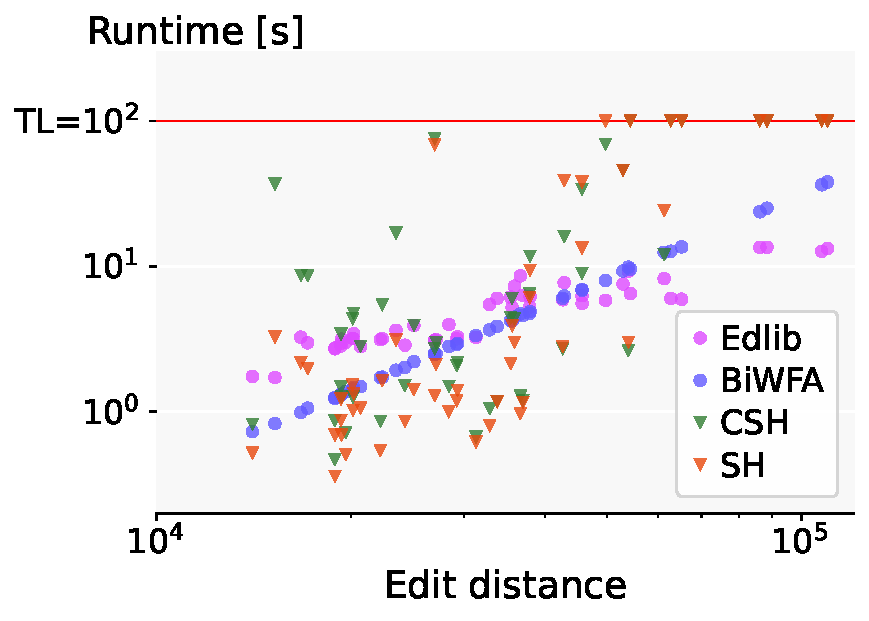
\includegraphics[width=0.48\linewidth]{imgs/fig7/human_chm13.pdf}}
  \hfill
  \subfloat[NA12878]{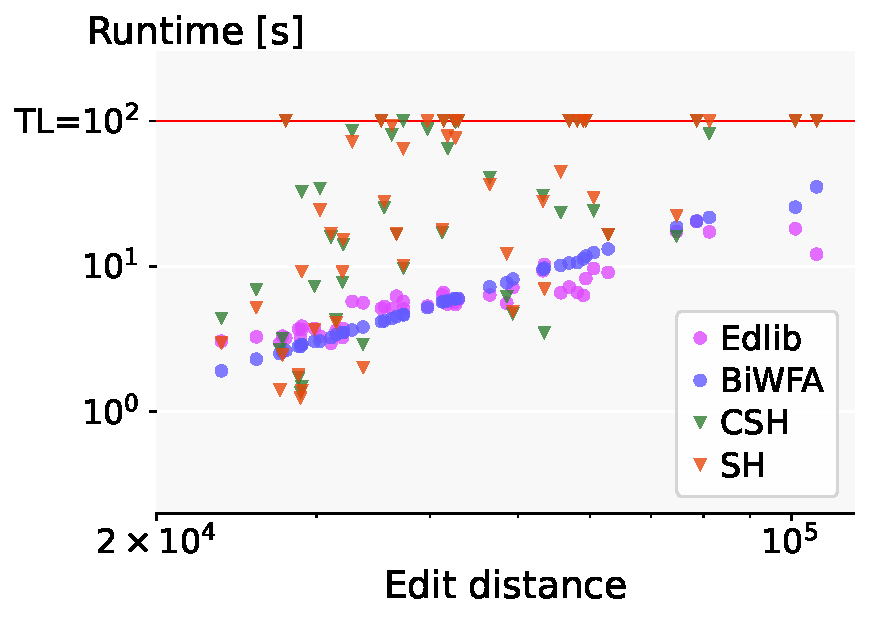
\includegraphics[width=0.48\linewidth]{imgs/fig7/human_na12878.pdf}}
  \caption[Runtime scaling with alignment cost]{Log-log plots of the runtime for aligning \textbf{real sequences}
  from two datasets of varying error distance. The sequence length varies
  between $500\kbp$ and $840\kbp$ for the CHM13 reads, and between $502\kbp$ and
  $1\ 053\kbp$ for the NA12878 reads. Alignments that timed out after $100$
  seconds are shown at $\qty{100}{s}$. Parameters used for SH and CSH are
  $k{=}15$ and $r{=}2$.}
  \label{GLOBALfig:human-results-unsorted}
\end{figure}

% biwfa and edlib
Note that the \wfa data points lie on a line, corresponding to the
expected runtime of \wfa of $\Oh(s^2)$. Furthermore, the runtime of \edlib can be
seen to jump up around powers of two ($2^{14} {=} 16\,384$, $2^{15} {=} 32\,768$,
$2^{16} {=} 65\,536$), corresponding to the exponential search of the edit
distance. \edlib has a runtime complexity of $\Oh(ns)$, and hence is slower than
\wfa for small edit distances, but faster than \wfa for large edit distances.
